% Options for packages loaded elsewhere
\PassOptionsToPackage{unicode}{hyperref}
\PassOptionsToPackage{hyphens}{url}
%
\documentclass[
  man]{apa7}
\usepackage{amsmath,amssymb}
\usepackage{lmodern}
\usepackage{iftex}
\ifPDFTeX
  \usepackage[T1]{fontenc}
  \usepackage[utf8]{inputenc}
  \usepackage{textcomp} % provide euro and other symbols
\else % if luatex or xetex
  \usepackage{unicode-math}
  \defaultfontfeatures{Scale=MatchLowercase}
  \defaultfontfeatures[\rmfamily]{Ligatures=TeX,Scale=1}
\fi
% Use upquote if available, for straight quotes in verbatim environments
\IfFileExists{upquote.sty}{\usepackage{upquote}}{}
\IfFileExists{microtype.sty}{% use microtype if available
  \usepackage[]{microtype}
  \UseMicrotypeSet[protrusion]{basicmath} % disable protrusion for tt fonts
}{}
\makeatletter
\@ifundefined{KOMAClassName}{% if non-KOMA class
  \IfFileExists{parskip.sty}{%
    \usepackage{parskip}
  }{% else
    \setlength{\parindent}{0pt}
    \setlength{\parskip}{6pt plus 2pt minus 1pt}}
}{% if KOMA class
  \KOMAoptions{parskip=half}}
\makeatother
\usepackage{xcolor}
\usepackage{graphicx}
\makeatletter
\def\maxwidth{\ifdim\Gin@nat@width>\linewidth\linewidth\else\Gin@nat@width\fi}
\def\maxheight{\ifdim\Gin@nat@height>\textheight\textheight\else\Gin@nat@height\fi}
\makeatother
% Scale images if necessary, so that they will not overflow the page
% margins by default, and it is still possible to overwrite the defaults
% using explicit options in \includegraphics[width, height, ...]{}
\setkeys{Gin}{width=\maxwidth,height=\maxheight,keepaspectratio}
% Set default figure placement to htbp
\makeatletter
\def\fps@figure{htbp}
\makeatother
\setlength{\emergencystretch}{3em} % prevent overfull lines
\providecommand{\tightlist}{%
  \setlength{\itemsep}{0pt}\setlength{\parskip}{0pt}}
\setcounter{secnumdepth}{-\maxdimen} % remove section numbering
% Make \paragraph and \subparagraph free-standing
\ifx\paragraph\undefined\else
  \let\oldparagraph\paragraph
  \renewcommand{\paragraph}[1]{\oldparagraph{#1}\mbox{}}
\fi
\ifx\subparagraph\undefined\else
  \let\oldsubparagraph\subparagraph
  \renewcommand{\subparagraph}[1]{\oldsubparagraph{#1}\mbox{}}
\fi
\newlength{\cslhangindent}
\setlength{\cslhangindent}{1.5em}
\newlength{\csllabelwidth}
\setlength{\csllabelwidth}{3em}
\newlength{\cslentryspacingunit} % times entry-spacing
\setlength{\cslentryspacingunit}{\parskip}
\newenvironment{CSLReferences}[2] % #1 hanging-ident, #2 entry spacing
 {% don't indent paragraphs
  \setlength{\parindent}{0pt}
  % turn on hanging indent if param 1 is 1
  \ifodd #1
  \let\oldpar\par
  \def\par{\hangindent=\cslhangindent\oldpar}
  \fi
  % set entry spacing
  \setlength{\parskip}{#2\cslentryspacingunit}
 }%
 {}
\usepackage{calc}
\newcommand{\CSLBlock}[1]{#1\hfill\break}
\newcommand{\CSLLeftMargin}[1]{\parbox[t]{\csllabelwidth}{#1}}
\newcommand{\CSLRightInline}[1]{\parbox[t]{\linewidth - \csllabelwidth}{#1}\break}
\newcommand{\CSLIndent}[1]{\hspace{\cslhangindent}#1}
\ifLuaTeX
\usepackage[bidi=basic]{babel}
\else
\usepackage[bidi=default]{babel}
\fi
\babelprovide[main,import]{english}
% get rid of language-specific shorthands (see #6817):
\let\LanguageShortHands\languageshorthands
\def\languageshorthands#1{}
% Manuscript styling
\usepackage{upgreek}
\captionsetup{font=singlespacing,justification=justified}

% Table formatting
\usepackage{longtable}
\usepackage{lscape}
% \usepackage[counterclockwise]{rotating}   % Landscape page setup for large tables
\usepackage{multirow}		% Table styling
\usepackage{tabularx}		% Control Column width
\usepackage[flushleft]{threeparttable}	% Allows for three part tables with a specified notes section
\usepackage{threeparttablex}            % Lets threeparttable work with longtable

% Create new environments so endfloat can handle them
% \newenvironment{ltable}
%   {\begin{landscape}\centering\begin{threeparttable}}
%   {\end{threeparttable}\end{landscape}}
\newenvironment{lltable}{\begin{landscape}\centering\begin{ThreePartTable}}{\end{ThreePartTable}\end{landscape}}

% Enables adjusting longtable caption width to table width
% Solution found at http://golatex.de/longtable-mit-caption-so-breit-wie-die-tabelle-t15767.html
\makeatletter
\newcommand\LastLTentrywidth{1em}
\newlength\longtablewidth
\setlength{\longtablewidth}{1in}
\newcommand{\getlongtablewidth}{\begingroup \ifcsname LT@\roman{LT@tables}\endcsname \global\longtablewidth=0pt \renewcommand{\LT@entry}[2]{\global\advance\longtablewidth by ##2\relax\gdef\LastLTentrywidth{##2}}\@nameuse{LT@\roman{LT@tables}} \fi \endgroup}

% \setlength{\parindent}{0.5in}
% \setlength{\parskip}{0pt plus 0pt minus 0pt}

% Overwrite redefinition of paragraph and subparagraph by the default LaTeX template
% See https://github.com/crsh/papaja/issues/292
\makeatletter
\renewcommand{\paragraph}{\@startsection{paragraph}{4}{\parindent}%
  {0\baselineskip \@plus 0.2ex \@minus 0.2ex}%
  {-1em}%
  {\normalfont\normalsize\bfseries\itshape\typesectitle}}

\renewcommand{\subparagraph}[1]{\@startsection{subparagraph}{5}{1em}%
  {0\baselineskip \@plus 0.2ex \@minus 0.2ex}%
  {-\z@\relax}%
  {\normalfont\normalsize\itshape\hspace{\parindent}{#1}\textit{\addperi}}{\relax}}
\makeatother

% \usepackage{etoolbox}
\makeatletter
\patchcmd{\HyOrg@maketitle}
  {\section{\normalfont\normalsize\abstractname}}
  {\section*{\normalfont\normalsize\abstractname}}
  {}{\typeout{Failed to patch abstract.}}
\patchcmd{\HyOrg@maketitle}
  {\section{\protect\normalfont{\@title}}}
  {\section*{\protect\normalfont{\@title}}}
  {}{\typeout{Failed to patch title.}}
\makeatother

\usepackage{xpatch}
\makeatletter
\xapptocmd\appendix
  {\xapptocmd\section
    {\addcontentsline{toc}{section}{\appendixname\ifoneappendix\else~\theappendix\fi\\: #1}}
    {}{\InnerPatchFailed}%
  }
{}{\PatchFailed}
\keywords{AI, Students, Mental Health, Products\newline\indent Word count: X}
\DeclareDelayedFloatFlavor{ThreePartTable}{table}
\DeclareDelayedFloatFlavor{lltable}{table}
\DeclareDelayedFloatFlavor*{longtable}{table}
\makeatletter
\renewcommand{\efloat@iwrite}[1]{\immediate\expandafter\protected@write\csname efloat@post#1\endcsname{}}
\makeatother
\usepackage{lineno}

\linenumbers
\usepackage{csquotes}
\makeatletter
\renewcommand{\paragraph}{\@startsection{paragraph}{4}{\parindent}%
  {0\baselineskip \@plus 0.2ex \@minus 0.2ex}%
  {-1em}%
  {\normalfont\normalsize\bfseries\typesectitle}}
\renewcommand{\subparagraph}[1]{\@startsection{subparagraph}{5}{1em}%
  {0\baselineskip \@plus 0.2ex \@minus 0.2ex}%
  {-\z@\relax}%
  {\normalfont\normalsize\bfseries\itshape\hspace{\parindent}{#1}\textit{\addperi}}{\relax}}
\makeatother

\ifLuaTeX
  \usepackage{selnolig}  % disable illegal ligatures
\fi
\IfFileExists{bookmark.sty}{\usepackage{bookmark}}{\usepackage{hyperref}}
\IfFileExists{xurl.sty}{\usepackage{xurl}}{} % add URL line breaks if available
\urlstyle{same} % disable monospaced font for URLs
\hypersetup{
  pdftitle={Students' attitudes towards AI in Psychiatry},
  pdfauthor={Anne-Kathrin Kleine1 \& },
  pdflang={en-EN},
  pdfkeywords={AI, Students, Mental Health, Products},
  hidelinks,
  pdfcreator={LaTeX via pandoc}}

\title{Students' attitudes towards AI in Psychiatry}
\author{Anne-Kathrin Kleine\textsuperscript{1} \& \textsuperscript{}}
\date{}


\shorttitle{AI in Psychiatry}

\authornote{

LMU

The authors made the following contributions. Anne-Kathrin Kleine: Conceptualization, Writing - Original Draft Preparation, Writing - Review \& Editing; : , .

Correspondence concerning this article should be addressed to Anne-Kathrin Kleine, . E-mail: \href{mailto:Anne-Kathrin.Kleine@psy.lmu.de}{\nolinkurl{Anne-Kathrin.Kleine@psy.lmu.de}}

}

\affiliation{\vspace{0.5cm}\textsuperscript{1} LMU\\\textsuperscript{} }

\begin{document}
\maketitle

\hypertarget{introduction}{%
\section{Introduction}\label{introduction}}

The application of AI technology in mental healthcare is on the rise Jiang et al. (2017).
Although many applications are still in development, several AI products that aid in diagnosing and treating mental illnesses, selecting appropriate treatment approaches, predicting treatment success, and improving psycho-therapeutic interventions are already available to mental health professionals Cummins et al. (2019).
Given the large number of registered patents related to identifying and diagnosing psychiatric illnesses, the number of AI applications in the mental health sector may be expected to increase further over the following years (Zheng et al., 2022).

\hypertarget{the-application-of-ai-technology-in-mental-health-care}{%
\section{The application of AI technology in mental health care}\label{the-application-of-ai-technology-in-mental-health-care}}

The application of AI technology in mental healthcare ranges from selecting appropriate treatment regimens to supporting therapist skill development.
In their scoping review of machine learning in psychotherapy research, Aafjes-van Doorn et al. (2021) identified 51 studies that developed and tested a machine learning algorithm focused on selecting appropriate treatment regimes, predicting treatment adherence and response, and therapist skill development.
Shatte et al. (2019) identified 190 mental health tools focused on detecting and diagnosing mental health conditions, 67 on prognosis, treatment, and support, 26 on public health applications, and 17 on research and clinical administration.
In the following, we provide a brief overview of how AI technology is used in the areas of a) assistance with detection, diagnosis, and prognosis, b) assistance with treatment and treatment selection, and c) improvement of psychotherapy quality and therapist skill development.
Detailed descriptions of AI technologies relevant for clinical practice in the different areas of mental health care have been provided elsewhere (e.g., Lee et al., 2021).

\hypertarget{assistance-with-detection-diagnosis-and-prognosis}{%
\subsection{Assistance with detection, diagnosis, and prognosis}\label{assistance-with-detection-diagnosis-and-prognosis}}

\hypertarget{assistance-with-treatment-and-treatment-selection}{%
\subsection{Assistance with treatment and treatment selection}\label{assistance-with-treatment-and-treatment-selection}}

\hypertarget{improvement-of-psychotherapy-quality}{%
\subsection{Improvement of psychotherapy quality}\label{improvement-of-psychotherapy-quality}}

Supervision and receiving performance-feedback on their therapy sessions supports psychotherapy trainees' acquisition of skills and increases retention Helge Rønnestad \& Ladany (2006).
However, the process of providing ongoing feedback is labor intensive and thus rarely used in training.
Feedback is often based on trainees' self-reports and usually only available long after the actual performance (Tanana et al., 2019).
Using artificial intelligence technology for training purposes in mental health care may leverage the problem by providing immediate and performance-specific feedback to psychotherapists and trainees.

Most of the tools developed to improve psychotherapy quality rely on natural language processing-based feedback Tanana et al. (2019).
For example, \emph{TIM} (Therapy Insights Model) uses real-time chat messages exchanged between therapists and patients to provide therapists with feedback regarding the topics that were sufficiently covered in the session and the topics that should be addressed in the next sessions (Cummins et al., 2019). \emph{CORE-MI} (Counselor Observer Ratings Expert for Motivational Interviewing uses audio recordings of motivational interviewing (MI) sessions to generate feedback on psychotherapists' adherence with MI principles.
The user receives feedback on six summary measures of MI fidelity: empathy, MI spirit, reflection-to-question ratio, percent open questions, percent complex reflections, and percent MI adherence.
\emph{CORE-MI} includes a visual summary of counseling sessions based on the fidelity assessment that may be used by the therapist to improve their MI performance (Hirsch et al., 2018). Similar tools include the \emph{ClientBot}, a training tool that mimics typical patient responses to therapist questions and provides real-time feedback on therapists' use of open questions and reflections (Tanana et al., 2019); or \emph{Partner}, a reinforcement learning agent that may increase the quality of mental health support conversations by suggesting sentence-level edits to posts that enhance the level of empathy while maintaining conversation quality (Sharma et al., 2021).

\hypertarget{reservations-against-the-application-of-ai-technology-in-mental-health-practice}{%
\section{Reservations against the application of AI technology in mental health practice}\label{reservations-against-the-application-of-ai-technology-in-mental-health-practice}}

Thus far, insight into healh practitioners' attitudes towards the application of AI technology is limited to the physical health domain, with inconclusive results Pinto dos Santos et al. (2019).
One study suggests that despite the strong belief in the efficiency of AI tools, only a minority (a quarter) of radiologists in the sample believed that AI tools can be trusted (Jungmann et al., 2020).
Other research findings suggest generally positive attitudes towards the application of AI in radiology (e.g., Codari et al., 2019).

Despite a large amount of research in the area of mental health AI technology, many of the algorithms developed and tested in research have not yet been integrated into clinical care (Sendak et al., 2020).
Reasons for this research-practice gap include technical difficulties and the black box problem of AI-based recommendations.
Technical difficulties primarily complicate the use of AI tools in diagnosis and prognosis and selecting treatment approaches. They encompass, for example, the inaccuracy of predictions, accuracy-interpretability tradeoffs, data privacy issues, and the difficulty of deriving clear-cut diagnoses in the light of ambiguous symptomatology or symptoms overlapping with other (mental) illnesses Aafjes-van Doorn et al. (2021).

In addition, is often not apparent to clinicians how AI-based recommendations are generated.
Despite the efforts made to enhance the explainability of AI recommendations, such as the Explainable Artificial Intelligence (XAI) Initiative, the complexity of deep learning approaches necessarily limits the extent to which they can be made accessible to a broader user group (Feldman et al., 2019).
Especially in the area of mental health care, where transparency and the explainability of clinical decision-making are highly valued, the black box problem of AI-based recommendations creates a significant obstacle against its adoption into clinical practice Kelly et al. (2019).

\hypertarget{reservations-against-the-application-of-ai-technology-in-mental-health-practice-among-medical-and-psychology-students}{%
\subsection{Reservations against the application of AI technology in mental health practice among medical and psychology students}\label{reservations-against-the-application-of-ai-technology-in-mental-health-practice-among-medical-and-psychology-students}}

\emph{Reserach Question 1}: Are there any differences in the attitude towards the application of AI technology in mental health care between medical students and psychology students?

\hypertarget{the-relationship-between-ai-knowledge-and-attitudes-towards-the-application-of-ai-technology-in-mental-health-care}{%
\section{The relationship between AI knowledge and attitudes towards the application of AI technology in mental health care}\label{the-relationship-between-ai-knowledge-and-attitudes-towards-the-application-of-ai-technology-in-mental-health-care}}

Technical difficulties concerning the generation of accurate predictions and a seamless adoption of AI tools into clinical practice may be and will be addressed by data scientists and mental health experts over the coming years.
It has been suggested that reluctance against the adoption of new technology remains high as long as there is a lack of understanding on the practitioner side (Feldman et al., 2019).

A basic understanding how AI recommendations are generated makes it easier for clinicians to a) explain their decisions to patients and stakeholders, b) make fewer errors in using the generated information in their practice, c) provide feedback to help improving AI-based diagnostic and treatment tools, d) improve their professional skills (Adadi \& Berrada, 2018).

\emph{Hypothesis 1:}: There is a positive relationship between the knowledge about AI tools used in a) assistance with detection, diagnosis, and prognosis, b) assistance with treatment and treatment selection, and c) improvement of psychotherapy quality and positive attitudes towards the application of AI technology in the respective area.

\hypertarget{the-moderating-role-of-need-satisfaction}{%
\section{The moderating role of need satisfaction}\label{the-moderating-role-of-need-satisfaction}}

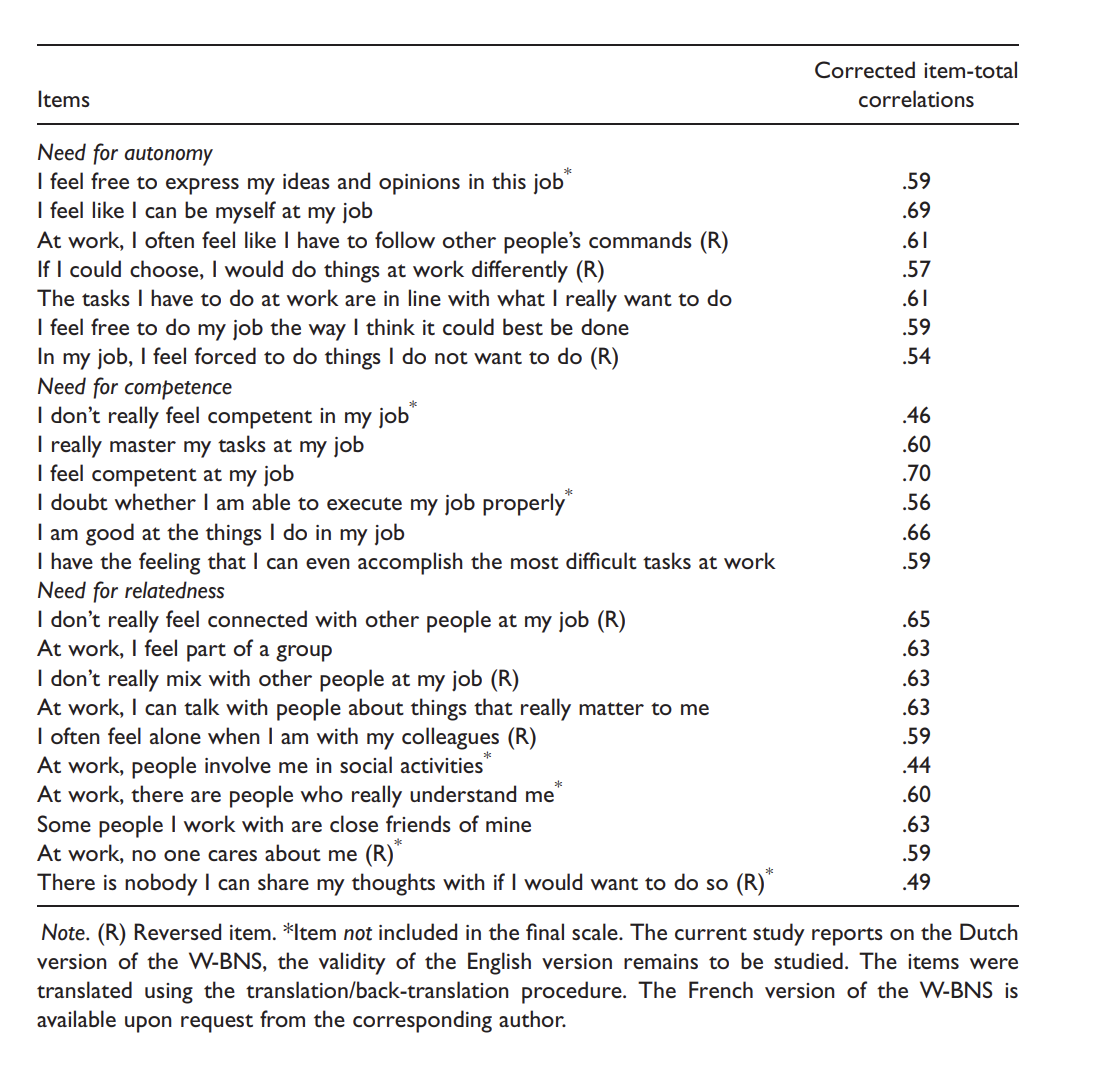
\includegraphics{../figs/need_sat.png}
- Idea: Adapt scale items to need satisfaction threat in future job; for example:
- ``I feel that AI tools used to {[}area of mental health{]} will make it more difficult to express my ideas and opinions in this job.''
- ``AI tools used to {[}area of mental health{]} will make it more difficult to be myself at my job.''

\emph{Hypothesis 2:}: The positive relationship between the knowledge about AI tools used in different mental health areas and positive attitudes towards the application of AI technology in these areas is attenuated by perceived threats to a) the need for autonomy, b) the need for competence, c) the need for relatedness posed by AI technology in the respective mental health area.

\hypertarget{other-ignore-part-below}{%
\subsection{OTHER (ignore part below)}\label{other-ignore-part-below}}

\hypertarget{attitudes-towards-ai-in-radiology}{%
\subsubsection{Attitudes towards AI in radiology}\label{attitudes-towards-ai-in-radiology}}

\begin{itemize}
\tightlist
\item
  The first section was aimed at evaluating whether the students had already heard
  of deep learning and AI in the context of radiology and whether they felt they had a basic grasp of the underlying technologies
\item
  The second section was introduced with a statement that AI is already being employed in relatively common software such as speech- and text-recognition, spam-filters and recommendation algorithms. The respondents were then asked to state whether or not they had already heard this in the media, on social media, during lectures or from friends/family
\item
  In the third and fourth sections, the students were presented with various statements and asked to indicate their level of agreement on a four-point Likert scale (disagree entirely, rather disagree, rather agree, or agree entirely). While the third section aimed at specific possible applications of AI in radiology, the fourth section had a broader scope and tried to assess the students' general fear of algorithms replacing human radiologists and other physicians.
\item
  The last section consisted of questions regarding respondent demographics as well as one question regarding whether the respondents considered themselves tech-savvy or not
\end{itemize}

\hypertarget{recruitment}{%
\subsubsection{Recruitment}\label{recruitment}}

\begin{itemize}
\tightlist
\item
  (\textbf{pintodossantosMedicalStudentsAttitude2019?}):

  \begin{itemize}
  \tightlist
  \item
    The questionnaire was sent out via email and advertised on social media to undergraduate medical students at three major German universities (University of Cologne, University of Bonn, University of Mainz). Participation was voluntary and had no relation to the students' curricular activities. The students were informed that the results of the survey would be used for further statistical evaluation and scientific publication. Respondent anonymity was guaranteed by design.
  \end{itemize}
\end{itemize}

\newpage

\hypertarget{references}{%
\section{References}\label{references}}

\hypertarget{refs}{}
\begin{CSLReferences}{1}{0}
\leavevmode\vadjust pre{\hypertarget{ref-aafjes-vandoorn_etal21}{}}%
Aafjes-van Doorn, K., Kamsteeg, C., Bate, J., \& Aafjes, M. (2021). A scoping review of machine learning in psychotherapy research. \emph{Psychotherapy Research}, \emph{31}(1), 92--116. \url{https://doi.org/10.1080/10503307.2020.1808729}

\leavevmode\vadjust pre{\hypertarget{ref-adadi_berrada18}{}}%
Adadi, A., \& Berrada, M. (2018). Peeking {Inside} the {Black}-{Box}: {A} {Survey} on {Explainable} {Artificial} {Intelligence} ({XAI}). \emph{IEEE Access}, \emph{6}, 52138--52160. \url{https://doi.org/10.1109/ACCESS.2018.2870052}

\leavevmode\vadjust pre{\hypertarget{ref-atkins_etal14}{}}%
Atkins, D. C., Steyvers, M., Imel, Z. E., \& Smyth, P. (2014). Scaling up the evaluation of psychotherapy: Evaluating motivational interviewing fidelity via statistical text classification. \emph{Implementation Science: IS}, \emph{9}, 49. \url{https://doi.org/10.1186/1748-5908-9-49}

\leavevmode\vadjust pre{\hypertarget{ref-can_etal16}{}}%
Can, D., Marín, R. A., Georgiou, P. G., Imel, Z. E., Atkins, D. C., \& Narayanan, S. S. (2016). "{It} sounds like...": {A} natural language processing approach to detecting counselor reflections in motivational interviewing. \emph{Journal of Counseling Psychology}, \emph{63}(3), 343--350. \url{https://doi.org/10.1037/cou0000111}

\leavevmode\vadjust pre{\hypertarget{ref-chekroud_etal21}{}}%
Chekroud, A. M., Bondar, J., Delgadillo, J., Doherty, G., Wasil, A., Fokkema, M., Cohen, Z., Belgrave, D., DeRubeis, R., Iniesta, R., Dwyer, D., \& Choi, K. (2021). The promise of machine learning in predicting treatment outcomes in psychiatry. \emph{World Psychiatry}, \emph{20}(2), 154--170. \url{https://doi.org/10.1002/wps.20882}

\leavevmode\vadjust pre{\hypertarget{ref-chen_etal22}{}}%
Chen, Z. S., Prathamesh, Kulkarni, Galatzer-Levy, I. R., Bigio, B., Nasca, C., \& Zhang, Y. (2022). \emph{Modern {Views} of {Machine} {Learning} for {Precision} {Psychiatry}}. arXiv. \url{http://arxiv.org/abs/2204.01607}

\leavevmode\vadjust pre{\hypertarget{ref-codari_etal19}{}}%
Codari, M., Melazzini, L., Morozov, S. P., Kuijk, C. C. van, Sconfienza, L. M., Sardanelli, F., \& European Society of Radiology (ESR). (2019). Impact of artificial intelligence on radiology: A {EuroAIM} survey among members of the {European} {Society} of {Radiology}. \emph{Insights into Imaging}, \emph{10}(1), 105. \url{https://doi.org/10.1186/s13244-019-0798-3}

\leavevmode\vadjust pre{\hypertarget{ref-cummins_etal19}{}}%
Cummins, R., Ewbank, M., Martin, A., Tablan, V., Catarino, A., \& Blackwell, A. (2019). \emph{{TIM}: {A} {Tool} for {Gaining} {Insights} into {Psychotherapy}}. \url{https://doi.org/10.1145/3308558.3314128}

\leavevmode\vadjust pre{\hypertarget{ref-feldman_etal19}{}}%
Feldman, R., Aldana, E., \& Stein, K. (2019). Artificial {Intelligence} in the {Health} care {Space}: {How} {We} {Can} {Trust} {What} {We} {Cannot} {Know}. \emph{Policy Review}, \emph{30}, 23. \url{https://repository.uchastings.edu/faculty_scholarship/1753/}

\leavevmode\vadjust pre{\hypertarget{ref-gong_etal19}{}}%
Gong, B., Nugent, J. P., Guest, W., Parker, W., Chang, P. J., Khosa, F., \& Nicolaou, S. (2019). Influence of {Artificial} {Intelligence} on {Canadian} {Medical} {Students}' {Preference} for {Radiology} {Specialty}: {ANational} {Survey} {Study}. \emph{Academic Radiology}, \emph{26}(4), 566--577. \url{https://doi.org/10.1016/j.acra.2018.10.007}

\leavevmode\vadjust pre{\hypertarget{ref-helgeronnestad_ladany06}{}}%
Helge Rønnestad, M., \& Ladany, N. (2006). The impact of psychotherapy training: {Introduction} to the special section. \emph{Psychotherapy Research}, \emph{16}(3), 261--267. \url{https://doi.org/10.1080/10503300600612241}

\leavevmode\vadjust pre{\hypertarget{ref-hirsch_etal18}{}}%
Hirsch, T., Soma, C., Merced, K., Kuo, P., Dembe, A., Caperton, D. D., Atkins, D. C., \& Imel, Z. E. (2018). {``{It}'s hard to argue with a computer:''} {Investigating} {Psychotherapists}' {Attitudes} towards {Automated} {Evaluation}. \emph{DIS. Designing Interactive Systems (Conference)}, \emph{2018}, 559--571. \url{https://doi.org/10.1145/3196709.3196776}

\leavevmode\vadjust pre{\hypertarget{ref-jiang_etal17}{}}%
Jiang, F., Jiang, Y., Zhi, H., Dong, Y., Li, H., Ma, S., Wang, Y., Dong, Q., Shen, H., \& Wang, Y. (2017). Artificial intelligence in healthcare: Past, present and future. \emph{Stroke and Vascular Neurology}, \emph{2}(4), 230--243. \url{https://doi.org/10.1136/svn-2017-000101}

\leavevmode\vadjust pre{\hypertarget{ref-jungmann_etal20}{}}%
Jungmann, F., Jorg, T., Hahn, F., Pinto dos Santos, D., Jungmann (geb. Görgen), S., Düber, C., Mildenberger, P., \& Kloeckner, R. (2020). Attitudes {Toward} {Artificial} {Intelligence} {Among} {Radiologists}, {IT} {Specialists}, and {Industry}. \emph{Academic Radiology}, \emph{28}. \url{https://doi.org/10.1016/j.acra.2020.04.011}

\leavevmode\vadjust pre{\hypertarget{ref-kelly_etal19}{}}%
Kelly, C. J., Karthikesalingam, A., Suleyman, M., Corrado, G., \& King, D. (2019). Key challenges for delivering clinical impact with artificial intelligence. \emph{BMC Medicine}, \emph{17}(1), 195. \url{https://doi.org/10.1186/s12916-019-1426-2}

\leavevmode\vadjust pre{\hypertarget{ref-lee_etal21}{}}%
Lee, E. E., Torous, J., De Choudhury, M., Depp, C. A., Graham, S. A., Kim, H.-C., Paulus, M. P., Krystal, J. H., \& Jeste, D. V. (2021). Artificial {Intelligence} for {Mental} {Health} {Care}: {Clinical} {Applications}, {Barriers}, {Facilitators}, and {Artificial} {Wisdom}. \emph{Biological Psychiatry: Cognitive Neuroscience and Neuroimaging}, \emph{6}(9), 856--864. \url{https://doi.org/10.1016/j.bpsc.2021.02.001}

\leavevmode\vadjust pre{\hypertarget{ref-megerian_etal22}{}}%
Megerian, J. T., Dey, S., Melmed, R. D., Coury, D. L., Lerner, M., Nicholls, C. J., Sohl, K., Rouhbakhsh, R., Narasimhan, A., Romain, J., Golla, S., Shareef, S., Ostrovsky, A., Shannon, J., Kraft, C., Liu-Mayo, S., Abbas, H., Gal-Szabo, D. E., Wall, D. P., \& Taraman, S. (2022). Evaluation of an artificial intelligence-based medical device for diagnosis of autism spectrum disorder. \emph{Npj Digital Medicine}, \emph{5}(1), 57. \url{https://doi.org/10.1038/s41746-022-00598-6}

\leavevmode\vadjust pre{\hypertarget{ref-miller_brown18}{}}%
Miller, D. D., \& Brown, E. W. (2018). Artificial {Intelligence} in {Medical} {Practice}: {The} {Question} to the {Answer}? \emph{The American Journal of Medicine}, \emph{131}(2), 129--133. \url{https://doi.org/10.1016/j.amjmed.2017.10.035}

\leavevmode\vadjust pre{\hypertarget{ref-moyers_etal05}{}}%
Moyers, T. B., Martin, T., Manuel, J. K., Hendrickson, S. M. L., \& Miller, W. R. (2005). Assessing competence in the use of motivational interviewing. \emph{Journal of Substance Abuse Treatment}, \emph{28}(1), 19--26. \url{https://doi.org/10.1016/j.jsat.2004.11.001}

\leavevmode\vadjust pre{\hypertarget{ref-pintodossantos_etal19}{}}%
Pinto dos Santos, D., Giese, D., Brodehl, S., Chon, S. H., Staab, W., Kleinert, R., Maintz, D., \& Baeßler, B. (2019). Medical students' attitude towards artificial intelligence: A multicentre survey. \emph{European Radiology}, \emph{29}(4), 1640--1646. \url{https://doi.org/10.1007/s00330-018-5601-1}

\leavevmode\vadjust pre{\hypertarget{ref-roth_etal21}{}}%
Roth, C. B., Papassotiropoulos, A., Brühl, A. B., Lang, U. E., \& Huber, C. G. (2021). Psychiatry in the {Digital} {Age}: {A} {Blessing} or a {Curse}? \emph{International Journal of Environmental Research and Public Health}, \emph{18}(16), 8302. \url{https://doi.org/10.3390/ijerph18168302}

\leavevmode\vadjust pre{\hypertarget{ref-sendak_etal20}{}}%
Sendak, M. P., D'Arcy, J., Kashyap, S., Gao, M., Nichols, M., Corey, K., Ratliff, W., \& Balu, S. (2020). A {Path} for {Translation} of {Machine} {Learning} {Products} into {Healthcare} {Delivery}. \emph{EMJ Innovations}. \url{https://doi.org/10.33590/emjinnov/19-00172}

\leavevmode\vadjust pre{\hypertarget{ref-sharma_etal21}{}}%
Sharma, A., Lin, I. W., Miner, A. S., Atkins, D. C., \& Althoff, T. (2021). Towards {Facilitating} {Empathic} {Conversations} in {Online} {Mental} {Health} {Support}: {A} {Reinforcement} {Learning} {Approach}. \emph{Proceedings of the {Web} {Conference} 2021}, 194--205. \url{https://doi.org/10.1145/3442381.3450097}

\leavevmode\vadjust pre{\hypertarget{ref-shatte_etal19}{}}%
Shatte, A. B. R., Hutchinson, D. M., \& Teague, S. J. (2019). Machine learning in mental health: A scoping review of methods and applications. \emph{Psychological Medicine}, \emph{49}(9), 1426--1448. \url{https://doi.org/10.1017/S0033291719000151}

\leavevmode\vadjust pre{\hypertarget{ref-tanana_etal19}{}}%
Tanana, M. J., Soma, C. S., Srikumar, V., Atkins, D. C., \& Imel, Z. E. (2019). Development and {Evaluation} of {ClientBot}: {Patient}-{Like} {Conversational} {Agent} to {Train} {Basic} {Counseling} {Skills}. \emph{Journal of Medical Internet Research}, \emph{21}(7), e12529. \url{https://doi.org/10.2196/12529}

\leavevmode\vadjust pre{\hypertarget{ref-zheng_etal22}{}}%
Zheng, F., Wang, L., Zeng, Z., \& Wu, S. (2022). International {Technologies} on {Prevention} and {Treatment} of {Neurological} and {Psychiatric} {Diseases}: {Bibliometric} {Analysis} of {Patents}. \emph{JMIR Mental Health}, \emph{9}(2), e25238. \url{https://doi.org/10.2196/25238}

\end{CSLReferences}


\end{document}
